\section{Amplificatore di carica}

\begin{figure}[h]
	\centering
	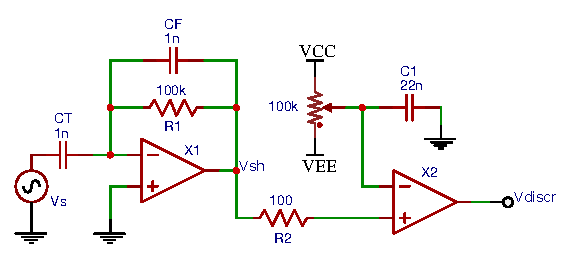
\includegraphics{charge-detector.pdf}
	\caption{Circuito rilevatore di carica.}
	\label{f:circ_qdet}
\end{figure}

Si è montato il circuito in \fig{circ_detq}, dove lo scopo del generatore di onde quadre $V_S$, insieme al condensatore $C_T$, è di iniettare nel nostro circuito una carica (che rappresenti ad esempio il segnale di un detector).

Il funzionamento che ci attendiamo, ammettendo l'idealità del generatore, dell'OpAmp e dei condensatori, è il seguente: al fronte di salita (o discesa) di $V_S$ una carica $\Delta V_S C_T$ si deposita sul condensatore $C_F$, portando dunque la tensione $V_{sh}$ a $\Delta V_S \frac{C_T}{C_F}$. La scarica del condensatore attraverso $R_1$ fa sì che la carica su di esso, e quindi la tensione $V_{sh}$, decadano esponenzialmente con un tempo caratteristico $\tau = C_F / R_1$. L'OpAmp $X_2$, configurato come discriminatore con una tensione di soglia positiva (vicina ai \SI{200}{\mV}), ha nel tempo in cui $V_{sh}$ è minore di tale soglia un'uscita $V_{discr}$ negativa ($\approx V_{EE}$); ai fronti di discesa di $V_S$ dunque non ci aspettiamo nessuna variazione dell'output (poichè $V_{sh}$ scende sotto lo 0), mentre ai fronti di salita dovremmo vedere $V_{discr}$ salire a $\approx V_{CC}$ e rimanerci fintantoché $V_{sh}$ non scenda, per lo scaricarsi del condensatore $C_F$, nuovamente al di sotto della tensione di soglia.
